\section{Examplary Two Player Game Sequence}
\subsection{Starting the Game}
As to be seen in Fig.\ref{fig:Starting2PlayerGame}, the main menu is created 
and added to the world by requet of the FBGame instance, returning the reference 
to the FBGame. This menu offers a few options to start a game session. Clicking 
on the "Start 2 Player Game" button results in the message 
\lstinline!FBGame>>startGames:! to be send with the parameter two. A loop is 
initialized, creating 2 discreet FBPlayfields by calling the 
\lstinline!createPlayfield: with:! method of FBWorld and linking the corresponding 
keymaps to them. A FBMultiplayerReward object is instantiated for the game.
%
\begin{figure}[bt]
  \begin{center}
    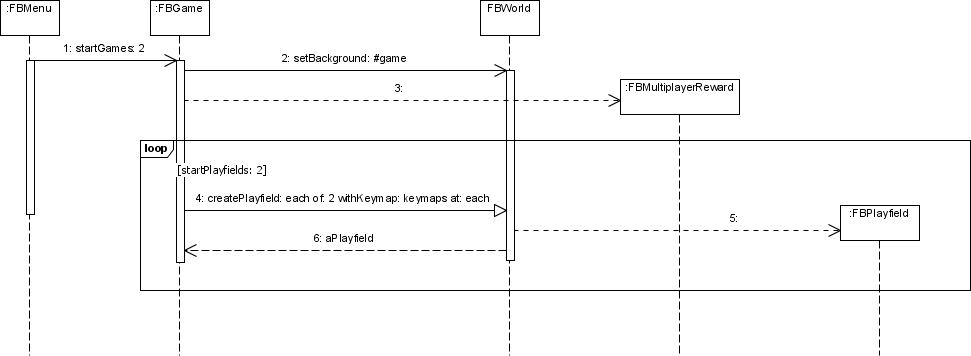
\includegraphics[width=\linewidth]{images/Starting2PlayerGame.png}
  \end{center}
  \caption{Starting a 2 Player Game}
  \label{fig:Starting2PlayerGame}
\end{figure}
%
%
\begin{figure}[bt]
  \begin{center}
    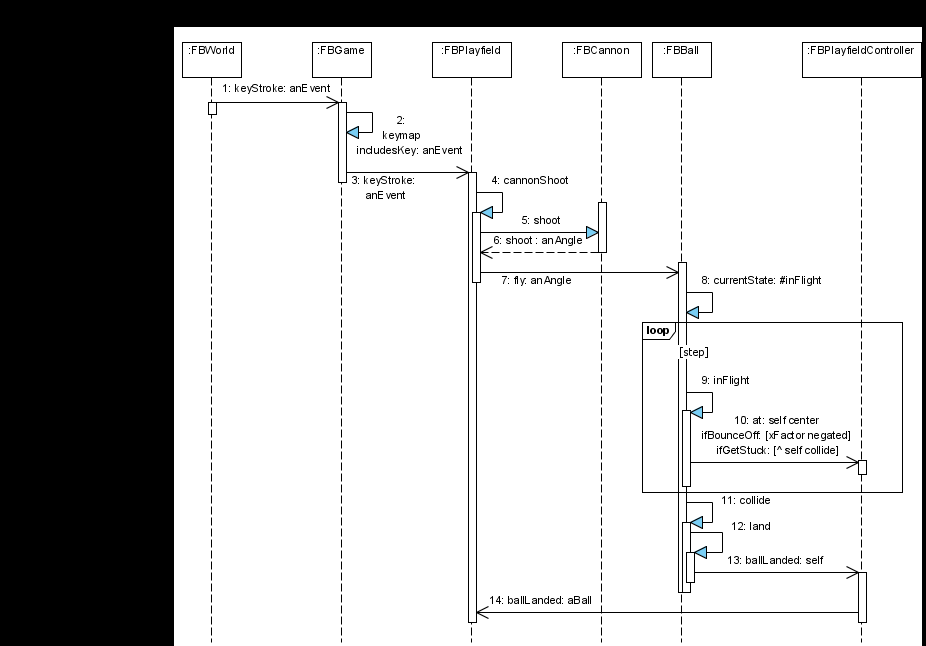
\includegraphics[width=\linewidth]{images/ShootingABall.png}
  \end{center}
  \caption{Shooting a Ball}
  \label{fig:ShootingABall}
\end{figure}
%
\subsection{Rewarding a Player}
Rewarding a player consists of very few steps, as depicted in Fig.\ref{fig:RewardingAPlayer}. 
First, the FBPlayfield of the player to be rewarded collects its reward 
through the \\{\lstinline!collectReward:!} method, thus calling the FBGame 
to distribute our reward. FBGame itself does not handle specific rewards 
itself, instead it informs the necessary FBRewardStrategy subclass, in 
this case FBMultiplayerReward, that a certain FBPlayfield needs to be 
rewarded. The bonus for a multiplayer playfield is actually a penalty 
for others, some FBBalls are randomly shot into the opponents playfield.

%
\begin{figure}[bt]
  \begin{center}
    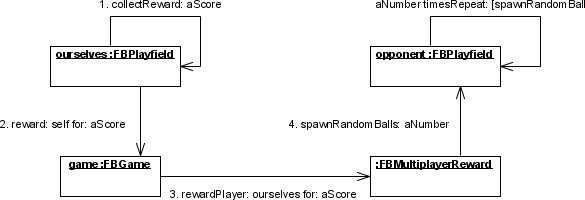
\includegraphics[width=\linewidth]{images/RewardingAPlayer.png}
  \end{center}
  \caption{Rewarding a Player for his Actions}
  \label{fig:RewardingAPlayer}
\end{figure}
%